\section{Numerical experiment}
\label{sec:experiment}

The experiments answer three questions, in this order: whether the trace is correct
(\S\ref{sec:exactness}); whether its speed on large problems comes from the structured
solve rather than from bookkeeping (\S\ref{sec:scaling}--\S\ref{sec:rankscaling}); and
how it compares with the alternatives, a QP swept over a grid and a parametric QP solver
(\S\ref{sec:clarabel}, \S\ref{sec:qpoases}). A real S\&P 500 frontier closes the section
(\S\ref{sec:empirical}); further checks are in Appendices~\ref{sec:details} and~\ref{sec:degeneracy}. Timings are
the median of three repetitions (bands span their range), each method and size in a
freshly spawned interpreter, on the machine of Computational details. Two complete runs
of the scaling sweep agree to within $10\%$ (median $3\%$) for traces of $10$~ms or more
and to within $40\%$ below that, so ratios are rounded accordingly and those at small
$n$ are indicative only.

\subsection{Correctness: a reference solver and a KKT certificate}
\label{sec:exactness}

On $40$ real assets (\S\ref{sec:empirical}; condition number $\approx 200$) the CLA
traces $29$ turning points. At the midpoint $\lambda$ of each of the $27$ interior
segments we re-solve \eqref{eq:qp} with \pkg{OSQP} \citep{stellato2020}, polished and
at tight tolerances, and compare with the interpolated CLA weights: the median
discrepancy is $2\times 10^{-15}$ and the maximum $6\times 10^{-8}$, solver precision
(\target{validate-exact}). Since each segment is
affine, one interior point certifies it. The step \target{validate-constraints}
validates two constrained frontiers the same way on a $30$-asset factor market: a budget plus
a neutrality row (the LP first vertex) and a budget with per-sector caps (an inequality
active at $30$ of $31$ turning points). Both match to $6\times 10^{-14}$ or better. A third
frontier is a $130/30$ book: the budget, shorts down to $-30\%$ per asset, and the
gross-exposure cap $\lVert w\rVert_1 \le 1.3$ of \S\ref{sec:leverage}, which binds at
$32$ of $49$ turning points; it matches to $1.4\times 10^{-12}$. The reference QP models
the cap with auxiliary variables $t \ge \lvert w\rvert$, independently of the lift.

A reference solver only shows that two codes agree; a KKT certificate tests the trace
itself (\target{validate-kkt}). At three interior points of every segment, and at two
values of $\lambda$ above the first turning point, the active set is read off the
interpolated weights (within $10^{-9}$ of a bound or of $h$), the multipliers are solved
from stationarity on the free coordinates, and primal feasibility, stationarity, dual
feasibility and complementary slackness are each measured. Neither the multipliers nor
the partition come from \pkg{cvxcla}, and the certificate always uses an explicit dense
$\Sig$, never the backend that traced the frontier. Where the free coordinates do not
determine the multipliers, at a vertex with no free weight, a bounded least-squares fit
asks whether sign-feasible multipliers exist. Primal feasibility is absolute, the other
conditions relative to $\max(1, \lVert\Sig w\rVert_\infty,
\lambda\lVert\mu\rVert_\infty)$. Over $2257$ points on eight traces
(Table~\ref{tab:kkt}), including the incremental and factor backends, the general
constraints and the lifted $130/30$ problem, no residual exceeds $2\times10^{-13}$. The
test does detect errors: weights shifted by $10^{-3}$ give a residual of
$2.5\times10^{-7}$, and weights paired with the $\lambda$ of another segment
$3.3\times10^{-4}$.

\begin{table}[t]
\centering
\small
\setlength{\tabcolsep}{5pt}
\begin{tabular}{lrrrrrr}
\hline
Problem & cond$(\Sig)$ & points & primal & station. & dual & compl. \\
\hline
S\&P 500, $40$ assets & $2.1\times10^{2}$ & $83$ & $2\times10^{-16}$ & $4\times10^{-17}$ & $0$ & $4\times10^{-22}$ \\
S\&P 500, $494$ assets & $1.1\times10^{5}$ & $284$ & $3\times10^{-16}$ & $2\times10^{-14}$ & $0$ & $5\times10^{-27}$ \\
\quad incremental backend & $1.1\times10^{5}$ & $284$ & $7\times10^{-16}$ & $2\times10^{-14}$ & $0$ & $3\times10^{-23}$ \\
\quad last $600$ days & $4.7\times10^{5}$ & $335$ & $4\times10^{-16}$ & $2\times10^{-13}$ & $0$ & $3\times10^{-23}$ \\
Factor market, $320$ assets & $1.3\times10^{3}$ & $965$ & $3\times10^{-14}$ & $9\times10^{-14}$ & $0$ & $0$ \\
$30$ assets: & & & & & & \\
\quad neutrality row & $8.3\times10^{1}$ & $98$ & $5\times10^{-14}$ & $1\times10^{-15}$ & $0$ & $2\times10^{-15}$ \\
\quad sector caps & $8.3\times10^{1}$ & $89$ & $4\times10^{-15}$ & $2\times10^{-15}$ & $0$ & $1\times10^{-15}$ \\
\quad $130/30$ cap & $8.3\times10^{1}$ & $119$ & $4\times10^{-15}$ & $9\times10^{-16}$ & $3\times10^{-16}$ & $4\times10^{-15}$ \\
\hline
\end{tabular}
\caption{Largest KKT residual of each condition (primal feasibility, stationarity,
dual feasibility, complementarity) over all points tested on a trace. Primal feasibility
is absolute; the other three are relative to
$\max(1, \lVert\Sig w\rVert_\infty, \lambda\lVert\mu\rVert_\infty)$. The factor market is
traced with the factor backend and checked against its dense $\Sig$; the $130/30$ problem
is checked in its lifted long/short form. Produced by \target{validate-kkt}.}
\label{tab:kkt}
\end{table}

\subsection{Runtime versus problem size}
\label{sec:scaling}

We trace the full frontier for $n \in \{20, 40, \dots, 2560\}$ assets, each from a
ground-truth $K = 10$ factor model, so the dense and factor backends run the same loop
on the same $\Sig$ and differ only in the free-block solve (\target{scaling}). The free
set is not small: on this market it grows to all $n$ assets, with a median of $n/2$ over
the trace. With the roughly $n$ steps observed here, a dense trace is about $n$ solves
of $O(n_\F^3)$ each, $O(n^4)$ operations, while the per-step cost of the factor backend is $O(n_\F K^2 + nK)$, so
$O(n^2 K)$ in total. At small $n$ a step's fixed overhead hides both rates, and the two backends are at
parity up to $n\approx 80$. Over the largest four sizes ($320$ to $2560$) the fitted
exponents are $\approx 2.9$ for the dense backend and $\approx 1.4$ for the factor
backend (Figure~\ref{fig:scaling}), below the operation counts because per-step
overhead has not yet given way entirely to arithmetic. The factor backend is about $4\times$
faster at $n=640$, $11\times$ at $1280$ and $35\times$ at $n=2560$, where it traces the
$2561$ turning points in about $1.2$~s against $41$~s
(Figure~\ref{fig:scaling}).

The factor backend also never holds an $n\times n$ matrix. At $n=2560$ its covariance
takes $0.22$~MiB against $50$~MiB, and the trace's working memory, the
\code{tracemalloc} peak less what the finished trace retains, is $0.84$~MiB against
$100$~MiB (Python objects and NumPy buffers; BLAS workspace is not counted). The stored frontier, $n$ weights per turning
point, is $O(n^2)$, $50$~MiB at $n=2560$, for either backend.

For external context we time the \code{CLA} of \pkg{PyPortfolioOpt}
\citep{pyportfolioopt}, the most familiar open implementation, based on
\citet{bailey2013}. It scales like $\approx n^{3.4}$ and takes about $275$~s at
$n=640$, against $0.6$~s for \pkg{cvxcla}'s dense backend; most of that gap is how
that code organises its per-step work (Appendix~\ref{sec:baileydetail}), which
\S\ref{sec:baseline} separates from the gain of the structured solve. The two
agree at the minimum-variance endpoint but not along the whole frontier: two bugs make
\pkg{PyPortfolioOpt} drop genuine turning points (Appendix~\ref{sec:baileydetail}).

\begin{figure}[t]
\centering
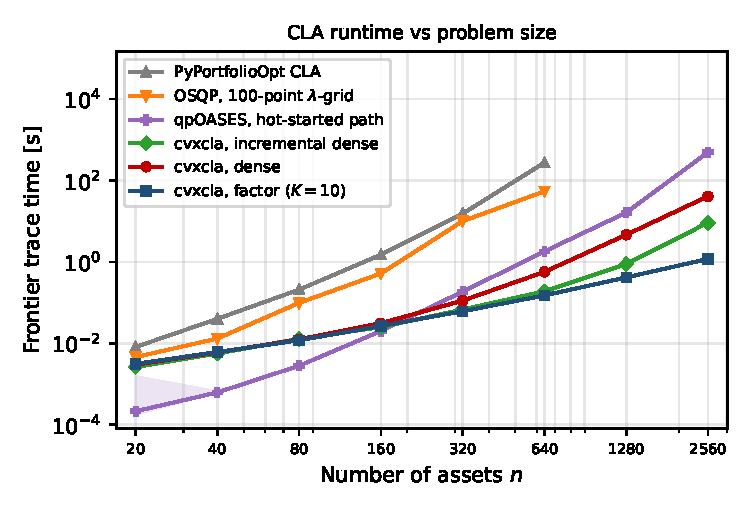
\includegraphics[width=0.54\textwidth]{scaling.pdf}
\caption{Frontier trace time against $n$ (log--log). Exponents $p$ of time $\approx n^p$,
fitted over the last four sizes each method was timed at with no overhead removed:
$2.9$ dense, $2.4$ incremental dense and $1.4$ factor ($n = 320$--$2560$), $3.4$
\pkg{PyPortfolioOpt} and $3.2$ \pkg{OSQP} ($80$--$640$), $3.7$ \pkg{qpOASES}
($320$--$2560$); they describe these sizes on this machine, not asymptotic complexity. \pkg{PyPortfolioOpt} and a warm-started \pkg{OSQP} grid of
$100$ values of $\lambda$ (\S\ref{sec:clarabel}) are timed up to $n=640$, and
\pkg{qpOASES} hot-started along the whole path (\S\ref{sec:qpoases}) up to $n=2560$.
The methods deliver different outputs: \pkg{cvxcla} and \pkg{PyPortfolioOpt} return
every turning point, the \pkg{OSQP} grid $100$ portfolios, and \pkg{qpOASES} only the
minimum-variance endpoint, so its time covers the path following alone.}
\label{fig:scaling}
\end{figure}

\subsection{Where the speed comes from}
\label{sec:baseline}

A fairer comparison sets \pkg{cvxcla}'s own dense backend against its opt-in
incremental one, \code{IncrementalDenseCovariance} (\S\ref{sec:incremental}), which runs the same loop
but maintains $\Sig_{\F\F}\inv$ by rank-one updates and reports the same turning points.
A trace is then $O(n^3)$, the measured exponent $\approx 2.4$, and the incremental
backend is about $3\times$ faster than the dense one at $n=640$ and $4.5\times$ at
$n=2560$: block elimination is not the fastest dense strategy. The factor backend is
still about $1.3\times$ faster than the incremental one at $n=640$ and $8\times$ at
$n=2560$, so the speed comes from the structured solve. Updating the Woodbury
capacitance $W$ incrementally would add little at $K=10$, where the $O(n)$ work of each
step (event scan, products with $\Sig$, bookkeeping) dominates, and matters only at
large $K$, where the dense backend is already faster (\S\ref{sec:rankscaling}).

\subsection{Runtime versus factor rank}
\label{sec:rankscaling}

The factor backend's advantage must fade as $K$ approaches $n$. At fixed $n = 320$ and
$K \in \{20, \dots, 320\}$ (\target{rank-scaling}), the dense time is flat in $K$ while Woodbury grows as
$O(n_\F K^2 + K^3)$: the factor backend is about $1.8\times$ faster at $K=20$, at parity near
$K=160$, and $\approx 1.7\times$ slower at $K = 320$. It pays off
in the regime real risk models inhabit, a few tens of factors over hundreds or thousands
of assets.

\subsection[A general-solver baseline: a QP swept over lambda]{A general-solver baseline: a QP swept over $\lambda$}
\label{sec:clarabel}

General toolkits (\pkg{Riskfolio-Lib} \citep{riskfolio}, \pkg{skfolio}
\citep{skfolio}, \pkg{fPortfolio} \citep{fportfolio}, \pkg{CVXR} \citep{cvxr}) hand a
single risk target to a general solver, so a frontier means re-solving \eqref{eq:qp} on
a grid. We make the grid as favourable as we can: \pkg{OSQP} \citep{stellato2020} is
set up once, each $\lambda$ changes only the linear term, and each solve warm-starts
from the last, over a fixed grid of $100$ values (\target{scaling}). The sweep grows
like $\approx n^{3.2}$ and is slower at every size, from about $1.5\times$ the dense
trace at $n=20$ to about $95\times$ at $n=640$ ($54$~s against $0.6$~s). On the
real frontier of \S\ref{sec:empirical} it is about $240\times$ slower at tolerance $10^{-6}$, and
at $10^{-5}$ it misses points by $10^{-3}$ (\target{osqp}). For a
single risk target a general solver is the natural choice; for the whole frontier on a
structured covariance, the trace is what separates \pkg{cvxcla} from these toolkits.

\subsection{A parametric QP solver}
\label{sec:qpoases}

\pkg{qpOASES} \citep{ferreau2014} solves parametric QPs by an online active-set
strategy: a hot start from one QP to the next follows the homotopy between them and
changes the working set at every breakpoint on the way. Hot-started from the
maximum-return end to $\lambda = 0$, it walks the same path as the CLA. We run it
through \pkg{CasADi} \citep{andersson2019}, solving once above the first finite turning
point and hot-starting once to $\lambda = 0$ (\target{scaling}).

The two codes follow the same path: \pkg{qpOASES} makes exactly as many working-set
changes as \pkg{cvxcla} reports turning points ($21, 42, \dots, 2561$), and its endpoint
matches the minimum-variance portfolio to $\sim\!2\times10^{-16}$. On small problems it
is faster, by a factor of several up to
$n=80$, where \pkg{cvxcla}'s \proglang{Python} per-step overhead dominates; the two meet
near $n=200$. Beyond that \pkg{qpOASES} grows like $\approx n^{3.7}$ and takes about $1.8$~s at
$n=640$ and $490$~s at $n=2560$: about $3\times$ and $12\times$ the dense backend, $12\times$
and $420\times$ the factor backend. It also returns only the endpoint, since the
turning points it passes are not exposed through the CasADi interface.

\subsection[Empirical example: the SP 500 frontier]{Empirical example: the S\&P 500 frontier}
\label{sec:empirical}

The experiment runs off a frozen snapshot shipped with the package:
$N = 494$ assets over $T = 1213$ trading days, 2021-07-30 to 2026-05-29, stored as
\srcfile{experiments/data/sp500_pct_returns.parquet}{sp500\_pct\_returns.parquet}
(SHA-256 \texttt{b5faa522\ldots9937e}) and produced once by
\srcfile{experiments/fetch_sp500.py}{fetch\_sp500.py}, retained for provenance only.
That script takes the index constituents listed on the day it was run, downloads their
split- and dividend-adjusted closes from \pkg{yfinance}, drops names missing more than
$5\%$ of the trading days, and forward-fills short gaps. The universe is the index at the end of the window, with survivorship bias, so we use it
only as a realistic covariance; it says nothing about investment performance. From the
full-history sample moments (condition number $\approx 1.1\times 10^{5}$) the CLA
traces the long-only frontier, $96$ turning points, in about $23$~ms;
a rank-$20$ factor approximation traces a
near-identical frontier ($89$ points) in about $15$~ms. The frontier spans annualised
returns of $0.14$--$0.89$ over volatilities of $0.10$--$0.87$, with an in-sample maximum
Sharpe ratio near $2.7$ (\target{real-frontier}).

\paragraph{Covariance estimators as backends.}
\label{sec:estimators}
Because \pkg{cvxcla} traces the frontier of whatever covariance it is given, a shrinkage
or factor estimate is simply another backend. Most remedies for a noisy sample
covariance \citep{johnstone2001} return the diagonal-plus-low-rank form
\eqref{eq:factor}: approximate factor models \citep{chamberlain1983}, POET
\citep{fan2013poet}, eigenvalue clipping \citep{laloux1999}, or Ledoit--Wolf shrinkage
\citep{ledoitwolf2004}, $(1-\rho)S + \rho F$. On the same universe, changing only the
covariance argument, \pkg{cvxcla} traces the frontier of the sample covariance ($96$
turning points), the Ledoit--Wolf estimate ($94$) and a rank-$20$ PCA model ($89$); the
three maximum-Sharpe portfolios hold $26$--$29$ names (\target{estimators}). As the
window shrinks past $T = n$ the sample covariance loses rank while the shrinkage and
factor estimates stay well-conditioned (\S\ref{sec:regularization}). \pkg{cvxcla}
controls only the computational error; an exact frontier of a noisy estimate is still
noisy, and ranking the estimators would take an out-of-sample study.

